\documentclass[12pt]{article}
\usepackage[margin=1in]{geometry}
\usepackage{graphicx}
\graphicspath{ {./} }


\title{Talkatiel Software Requirements and Planning}
\author{Brendan Byers, Ryan Sisco, Iliana J, Aidan Grimshaw}
\date{\today}

\begin{document}
\begin{center}
      \Large\textbf{User Stories and Set-up Assignment}\\
      \large\textit{Brendan Byers, Ryan Sisco, Iliana J, Aidan Grimshaw, Yufei Zeng}\\
      \large{byersbr, siscor, javieri, grimshaa, zengyu}\\
   \end{center}

\tableofcontents

\section{User Stories}

\subsection{Add a post}
As the user adds a post, his post body is checked for any illegal characters or
length, where it is then sent to the server and published.
\subsubsection{Corresponding Tasks}
This user story depends on getting an initial feed working.  Once the initial feed is complete, we can add the capability to add a post.  It will be due early on, as many other things depend on it.  Adding a post should be reasonably simple.  It will consist of a “post create” screen where a user writes their post.  When a button is clicked, the post will be verified and then sent to the server and added to the database.  Other users will then be able to view and react to it.  Paired programming time: 4 hours.

\subsubsection{UML Sequence Diagram/Spike}
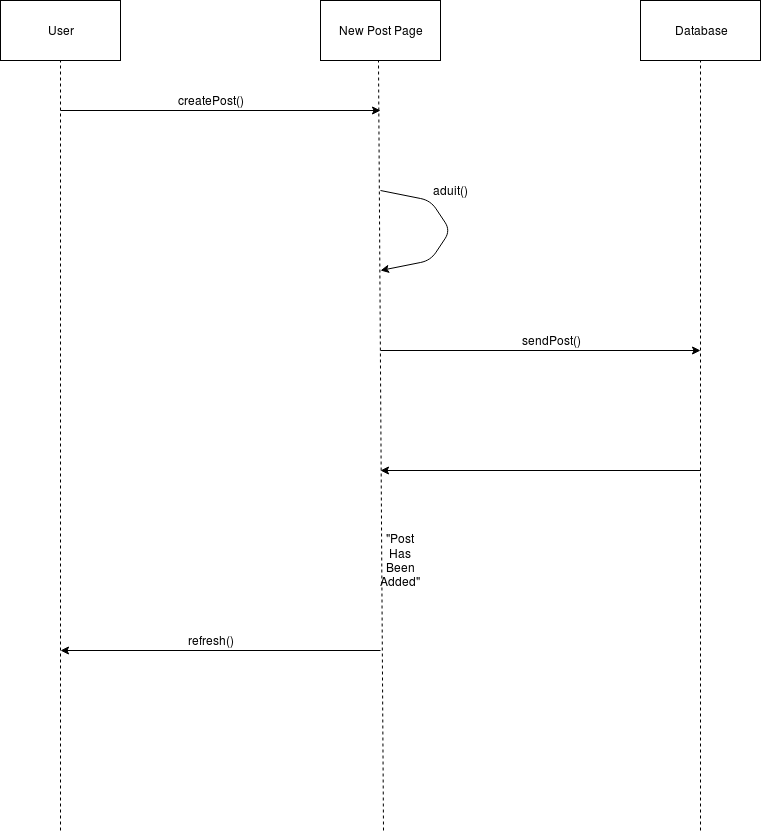
\includegraphics[scale=0.5]{img/story_1.png}\linebreak


\subsection{Add a comment}
When the user is on the post page, they can add a comment where it is checked
for any illegal characters or length, and then it is sent to the server and
published.
\begin{itemize}
  \item Response will be tied to the original post
  \item Responses aren’t viewable from the main feed
  \item Response can be voted on/shared/favorited
\end{itemize}
\subsubsection{Corresponding Tasks}
	This depends on the ability to create a post.  The process will be exactly the same, except when the comment is created it will be tied to the parent post.  Comments will behave exactly the same as posts.  This user story will be due after the ability to add a post is implemented.  Paired programming time: 2 hours.
\subsubsection{UML Sequence Diagram/Spike}
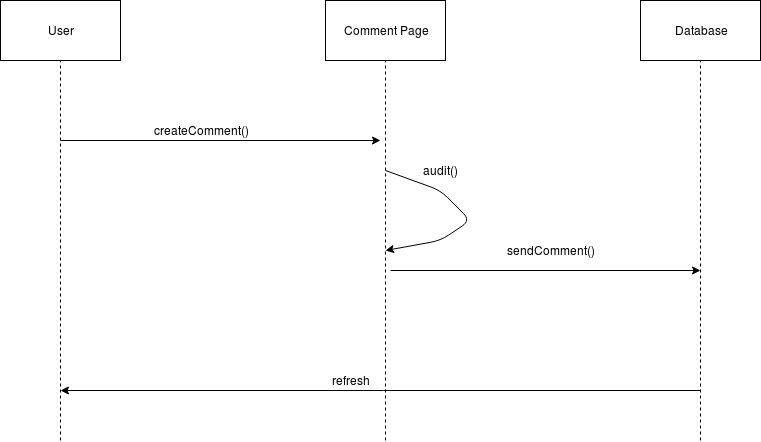
\includegraphics[scale=0.5]{img/story_2.png}\linebreak

\subsection{Like/Dislike}
When a user votes, their “+1” or “-1” is sent to the server, as long as they
have not voted on that post already, then the server is updated.
\begin{itemize}
  \item Posts can receive one vote from the user
  \item The user’s vote can be changed
  \item If a post is upvoted:
  \begin{itemize}
    \item If upvote is clicked the vote is removed
    \item If downvote is clicked the vote becomes a downvote
  \end{itemize}
\end{itemize}
\subsubsection{Corresponding Tasks}
	This user story depends on the “Add a Post” user story.  Once that is implemented we can begin work on this user story.  Buttons will be present on each post that when clicked enable to user to vote on a post.  The user can either like or dislike a post.  If a user previously liked a post and click like again, the vote is removed.  If dislike is clicked the post will be marked as so.  The total votes for a post should be stored server side.  Paired programming time: 6 hours.
\subsubsection{UML Sequence Diagram/Spike}
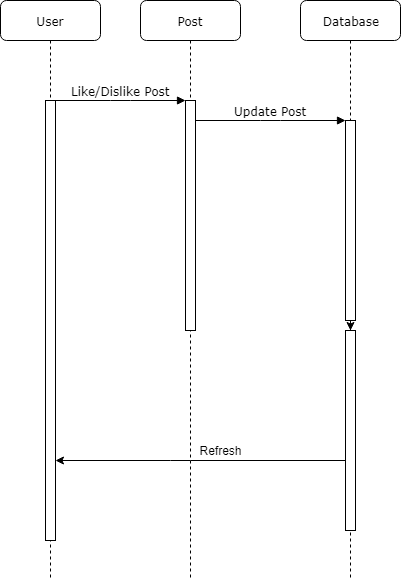
\includegraphics[scale=0.5]{img/3.png}\linebreak

\subsection{Report}
When a user clicks the report post button, the post is flagged for review. After
X amount of reports, the post is automatically taken down while waiting review.
\begin{itemize}
  \item When a user reports a post, the post won’t appear on the feed for that user
\end{itemize}
\subsubsection{Corresponding Tasks}
	This will be able to be completed once the post object has been created.  Users will click a button and a window will appear.  They will be able to choose or type in a reason for the reporting, then send the report.  When a post is reported by the user the post will be hidden from the users view indefinitely.  This depends on the functionality of the feed and refreshing posts.  Paired programming time: 6 hours.
\subsubsection{UML Sequence Diagram/Spike}
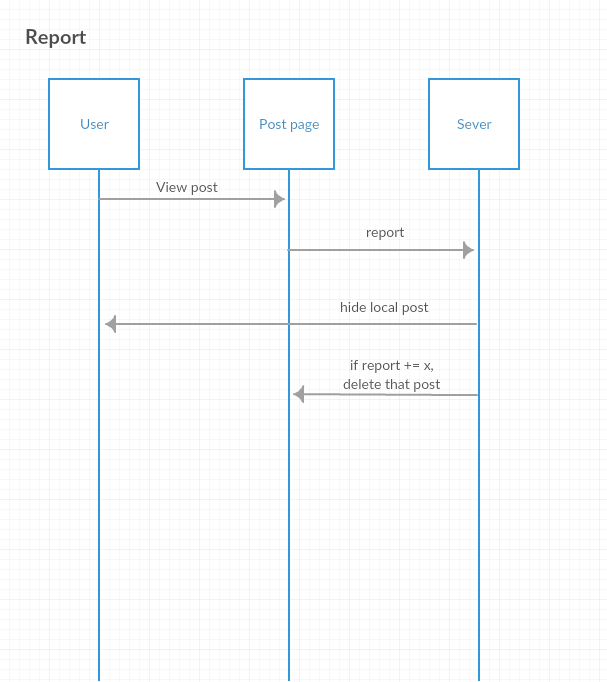
\includegraphics[scale=0.5]{img/4.png}\linebreak

\subsection{Delete}
When a user wants to delete a post, it is checked if it is their own post, if it
is, it is deleted. If it is not, it is checked if they are an admin, if they
are, it is deleted. The server will then update based on the above.
\subsubsection{Corresponding Tasks}
	This user story depends on the feed, posts, and refresh being implemented.  A button will be present on user created posts that allows them to delete their own posts.  This will allow people to delete what they posted before.  When a post is deleted it will no longer appear on any devices when the users refresh things.  Paired programming time: 5 hours.
\subsubsection{UML Sequence Diagram/Spike}
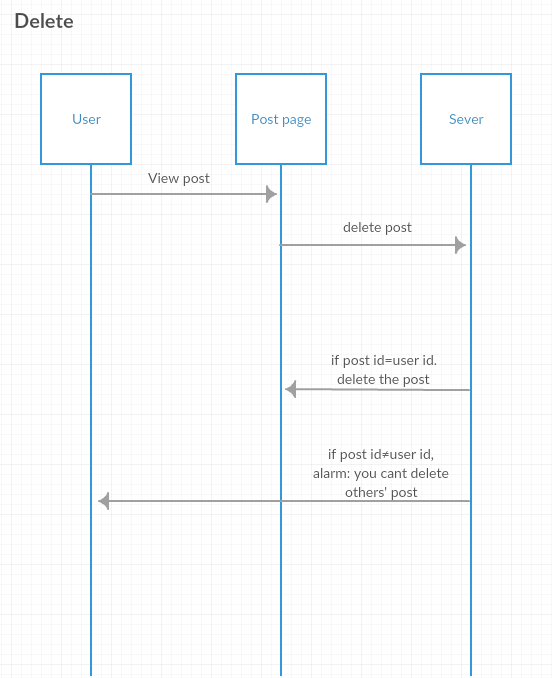
\includegraphics[scale=0.5]{img/5.png}\linebreak

\subsection{Refresh}
If the user swipes down on the screen, the page reacts with an animation and
then refreshes the page.
\subsubsection{Corresponding Tasks}
	This will be due after the implementation of posts and the feed.  This will refresh the feed and pull new posts from the database.  It won’t be a full refresh of the page.  IT will simply refresh the data within the page, giving a better user experience.  This will be a function of the service worker.  The new content will be fetched and then served to the user.  Paired programming time: 5 hours.
\subsubsection{UML Sequence Diagram/Spike}
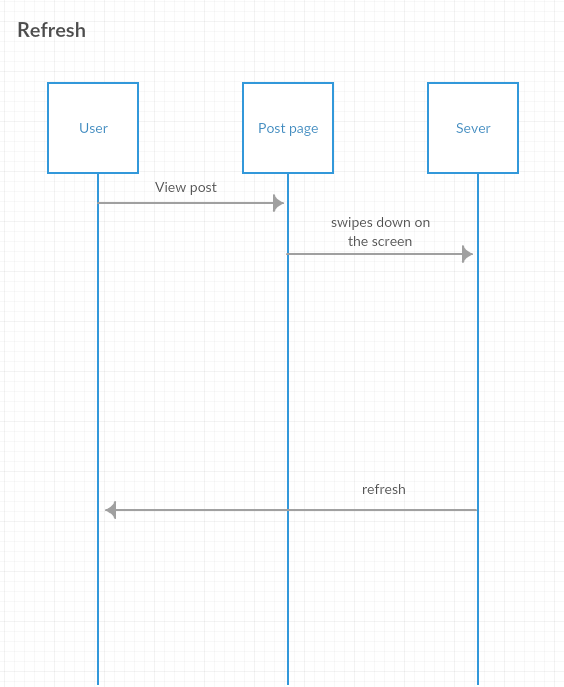
\includegraphics[scale=0.5]{img/6.png}\linebreak

\subsection{Sort}
when clicked, the page alerts the user of the sorting type and then changes the
sorting on the next click. They will be able to cycle through all of the
different types.
\subsubsection{Corresponding Tasks}
	Posts on the front page will be able to be sorted based on certain criteria.  Users will be able to sort based on top posts, new posts, and possibly hot posts.  This user story depends on the feed, post objects, and refreshing.  It will be due after refresh is implemented.  Paired Programming time: 3 hours.
\subsubsection{UML Sequence Diagram/Spike}
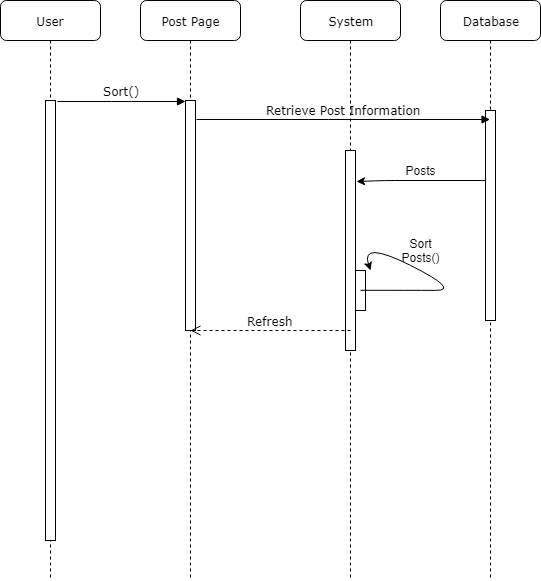
\includegraphics[scale=0.5]{img/7.png}\linebreak

\subsection{Add to Favorites}
All favorite posts are shown to the user by date added only.
\begin{itemize}
  \item After a post is added to favorited, the post on the main feed should show that
it is currently in the user’s favorites list
\end{itemize}
\subsubsection{Corresponding Tasks}
	This will enable a user to add a post to their favorites list.  It depends on the feed, posts, and favorites.  There will be a button on each post that allows the user to add that post to their favorites list.  When the button is clicked, the post will be saved in storage for viewing later.  The favorites list will not be stored server side. Paired Programming time: 5 hours.
\subsubsection{UML Sequence Diagram/Spike}
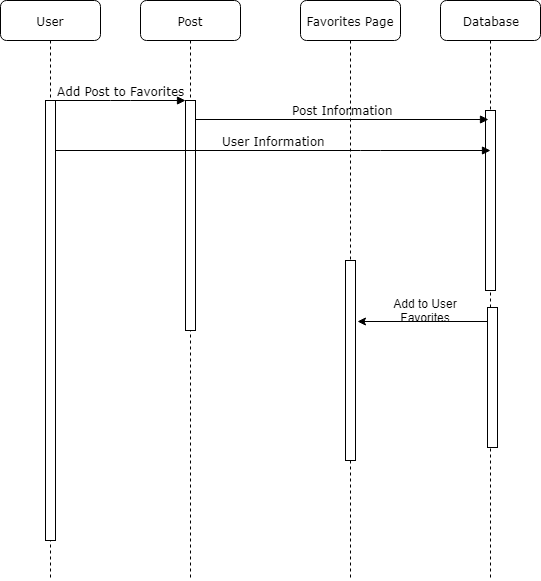
\includegraphics[scale=0.5]{img/8.png}\linebreak

\subsection{Offline Favorites}
When a user doesn’t have an internet connection, they should still be able to
see posts that they have favorited.
\begin{itemize}
  \item Store them in memory
  \item Posts will show instead of the “no internet” page
\end{itemize}
\subsubsection{Corresponding Tasks}
	This will enable the user to view their saved favorites while they are offline.  This will be due after offline capability and favorites are implemented.  The posts within the favorites list will be saved locally and viewed there.  Paired Programming time: 5 hours.
\subsubsection{UML Sequence Diagram/Spike}
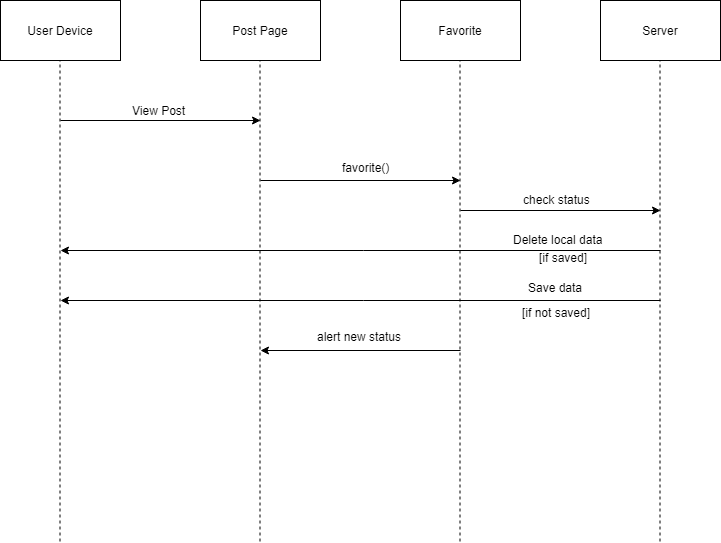
\includegraphics[scale=0.5]{img/9.png}\linebreak

\subsection{Offline Capability}
When a user is offline, they should be served a page telling them they have no
internet. All urls should load.
\begin{itemize}
  \item Use a service worker to monitor connections and requests
  \item If there’s no connection show a catch all page (exception is favorites page)
\end{itemize}
\subsubsection{Corresponding Tasks}
	This will enable to user to use the website when they have no internet connection.  IT will serve to simply show the user that they aren’t connected to the internet.  This is pretty easy to implement.  It depends on the ability to save websites as an app and the service worker.  Paired Programming time: 8 hours.
\subsubsection{UML Sequence Diagram/Spike}
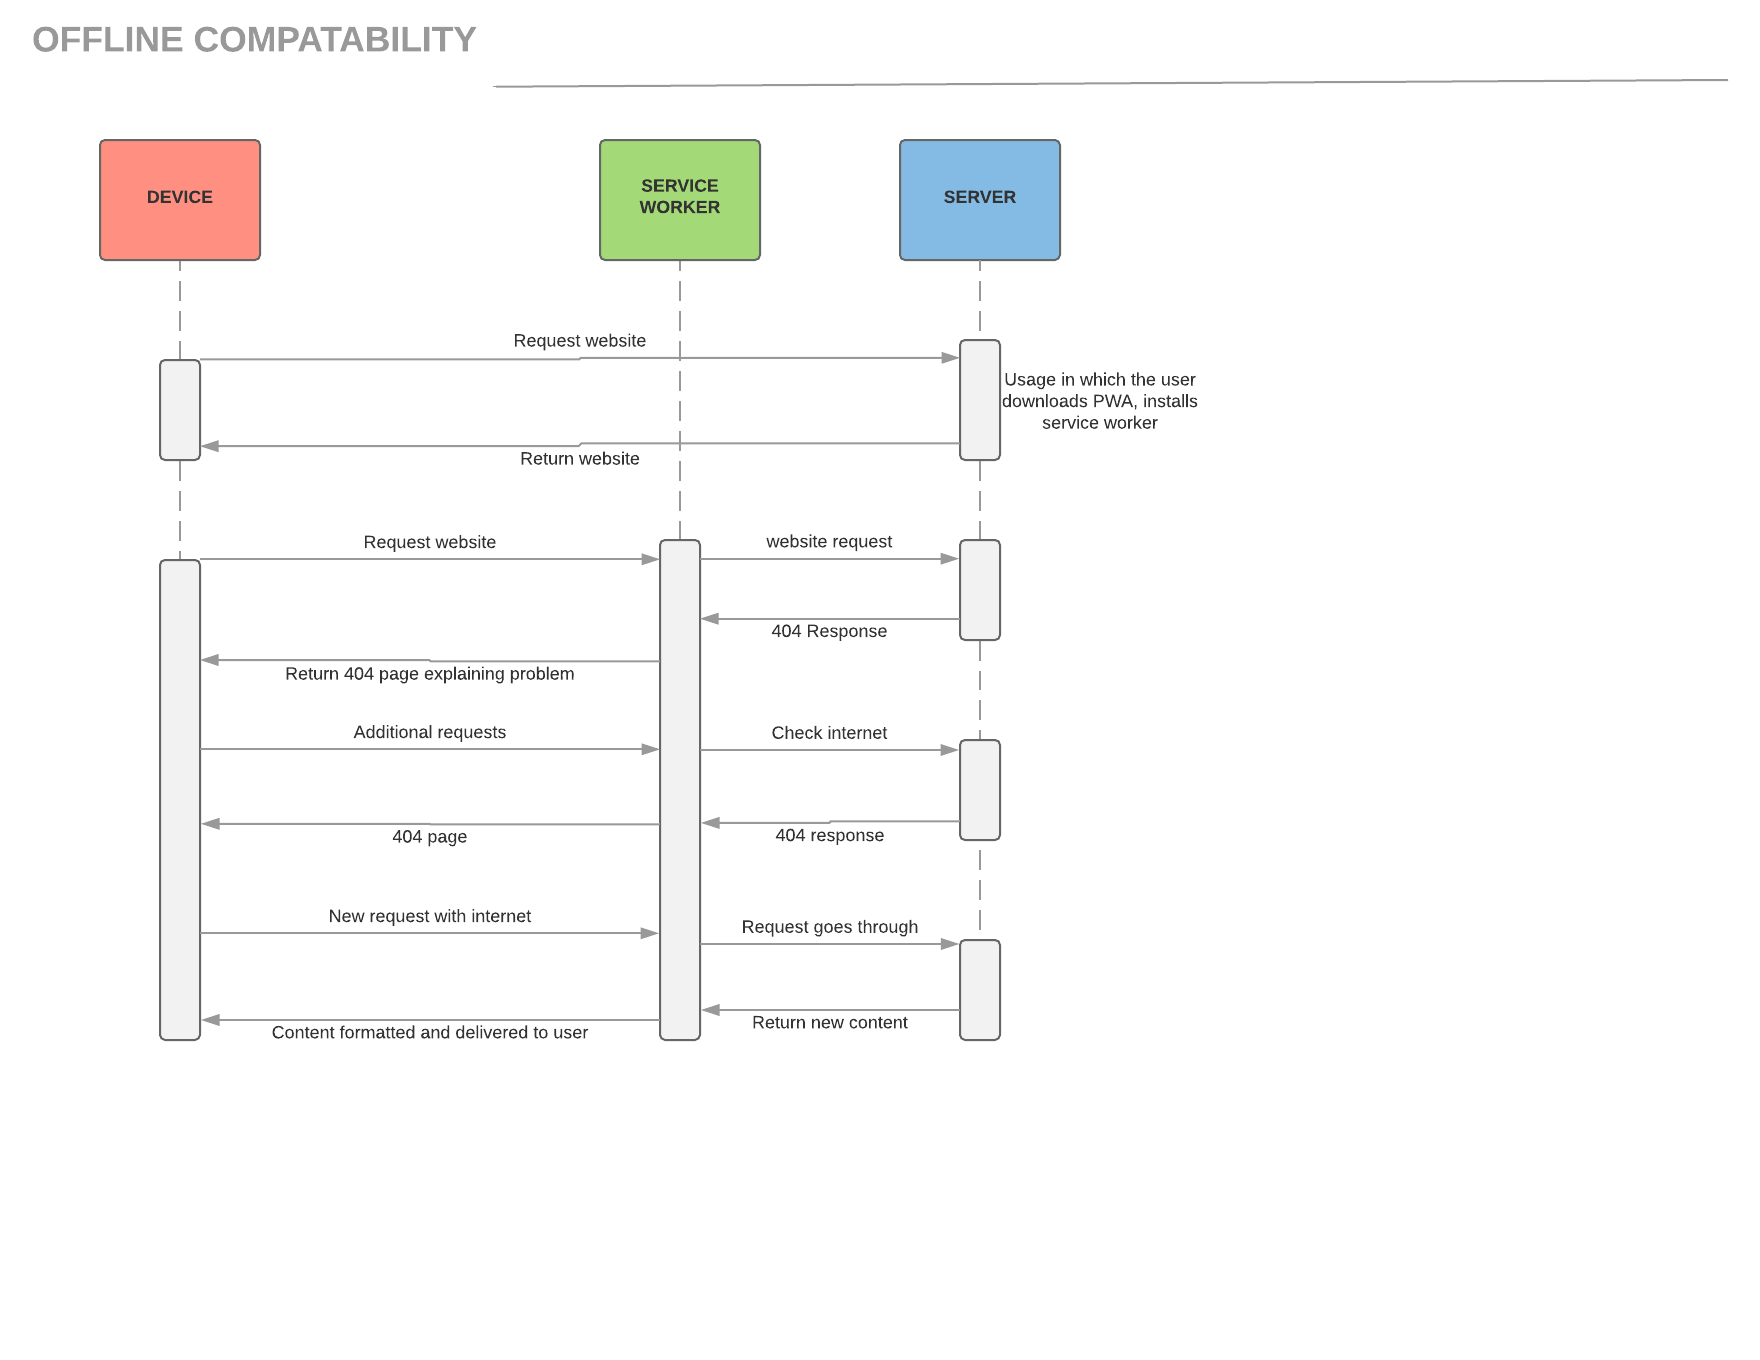
\includegraphics[scale=0.5]{img/10.png}\linebreak

\subsection{Browser Compatibility}
Web app should work in both chrome and safari.
\subsubsection{Corresponding Tasks}
	The PWA will work across different web browsers.  Our primary targets are safari on iOS and chrome on android.  Because this depends on the entire app, it will be due late in the development process once nearly everything is implemented.  This allows us to make things compatible all at once instead of continually needing to update things.  Paired Programming time: 4 hours.
\subsubsection{UML Sequence Diagram/Spike}

\subsection{View newly created Post}
When a post is created by a user, when they go back to the feed they should see
it immediately if sorted by new.
\subsubsection{Corresponding Tasks}
	When a user creates a post, they will be able to immediately see it at the top of their feed if it is sorted by “new”.  This user story depends on adding a post, adding a comment, refreshing, the feed, and sorting.  This is a low priority feature.  It will be due at the end, if at all.  Paired Programming time: 3 hours.
\subsubsection{UML Sequence Diagram/Spike}
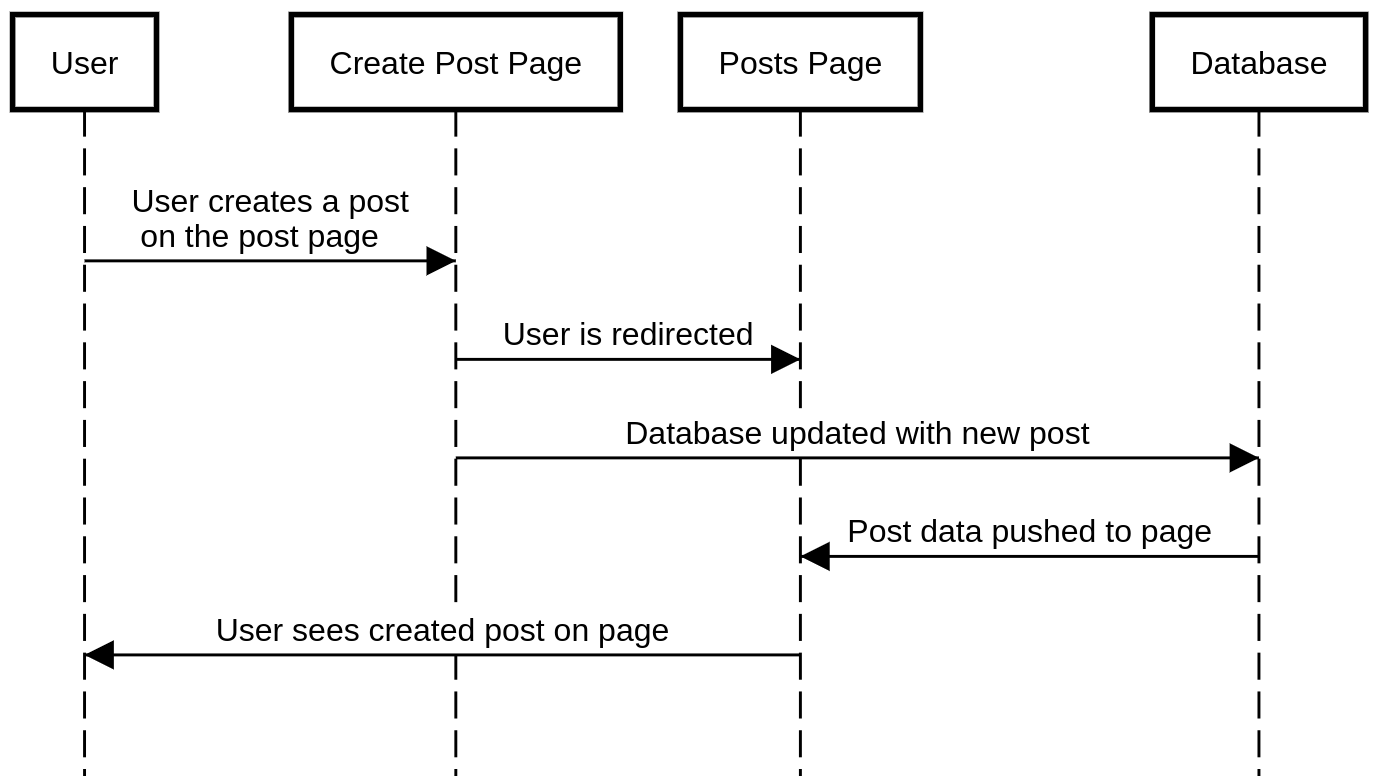
\includegraphics[scale=0.5]{img/view_newly_created_post.png}\linebreak

\subsection{Collapse Post Responses}
When viewing responses to a post, user should be able to collapse a response,
which will collapse that post and all the children.
\begin{itemize}
  \item Collapsing can be toggled by clicking on the response again
\end{itemize}
\subsubsection{Corresponding Tasks}
	When a user clicks on a post response/comment, the post should be able to collapse.  This will hide all the child comment to the response and make the clicked on response smaller.  When it is clicked on again it will return to original state.  This will serve to save space on the screen and hide what isn’t needed.  This user story depends on adding a post, adding a comment, refreshing, and the feed.  IT will be due pretty late as it is an enhancement.  Paired Programming time: 4 hours.
\subsubsection{UML Sequence Diagram/Spike}
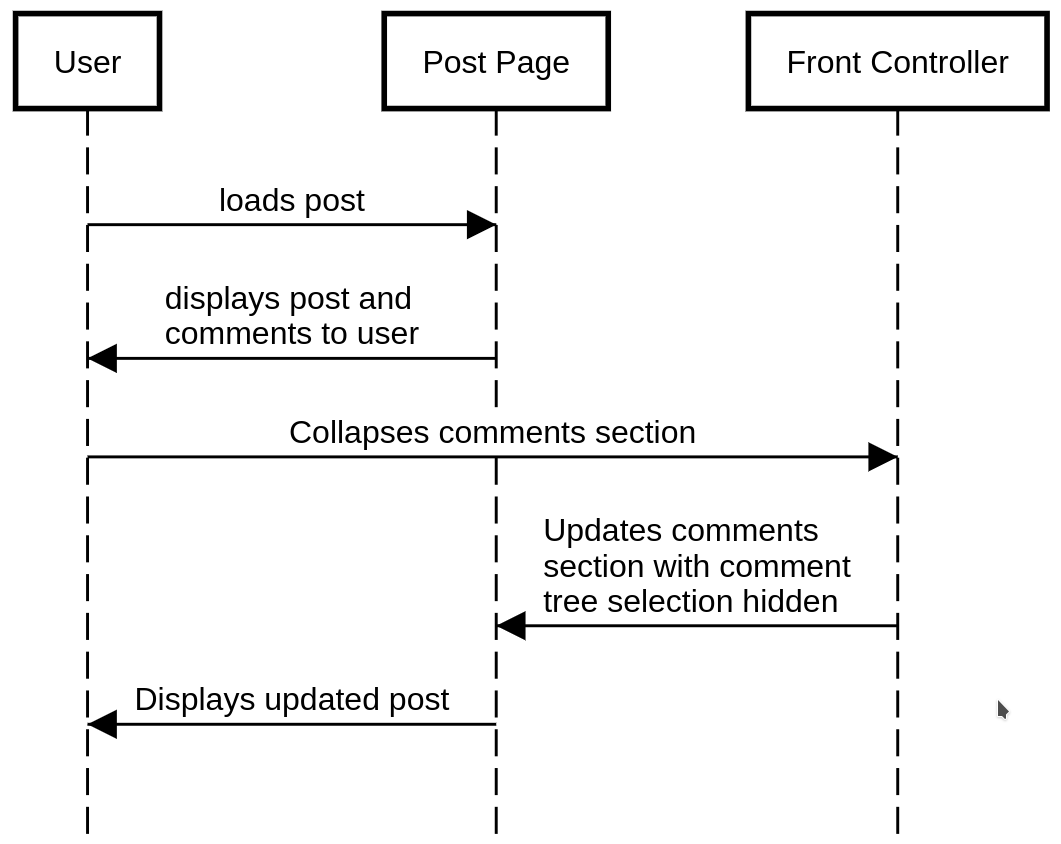
\includegraphics[scale=0.5]{img/collapse_post_responses.png}\linebreak

\subsection{Secure HTTPS}
All communication should be through an ssl connection.
\begin{itemize}
  \item Need a certificate from https://letsencrypt.org
\end{itemize}
\subsubsection{Corresponding Tasks}
	This consists of setting up the server that delivers content with a security certificate.  The certificate can be gotten from https://letsencrypt.org .  It will enable our server to deliver all content over https, improving security and following the guidelines of a PWA.  This will depend on the server side of things being implemented, which depends on the “Refresh” user story.  Paired Programming time: 4 hours.
\subsubsection{UML Sequence Diagram/Spike}

\subsection{Save Website as App on Phone}
Website should behave like a pwa and be able to be saved to a phones home screen.
\begin{itemize}
  \item Add a “web app manifest”
  \item Setup unique icons for the screen etc.
\end{itemize}
\subsubsection{Corresponding Tasks}
	This user story depends on the app manifest.  This is a document served with the website that tells the browser what the website is.  Ours will signal that it is a pwa and is able to be saved to the device.  This will depend on the service worker.  It will be due directly after the service worker is completed. Paired Programming time: 10 hours.
\subsubsection{UML Sequence Diagram/Spike}

\subsection{Responsive Web Page}
Content should scale with the size of the viewport/screen
\begin{itemize}
  \item Default viewport size should be defined in the app manifest
\end{itemize}
\subsubsection{Corresponding Tasks}
	The delivered web page should be responsive.  This means that as the screen size changes the content scales to best fit.  This can include removing flair or other things to save space.  This should only be needed for the desktop view, which will display a page saying to use a mobile device.  IT will depend on most of the rest of the project being complete.  Paired Programming time: 6 hours.
\subsubsection{UML Sequence Diagram/Spike}
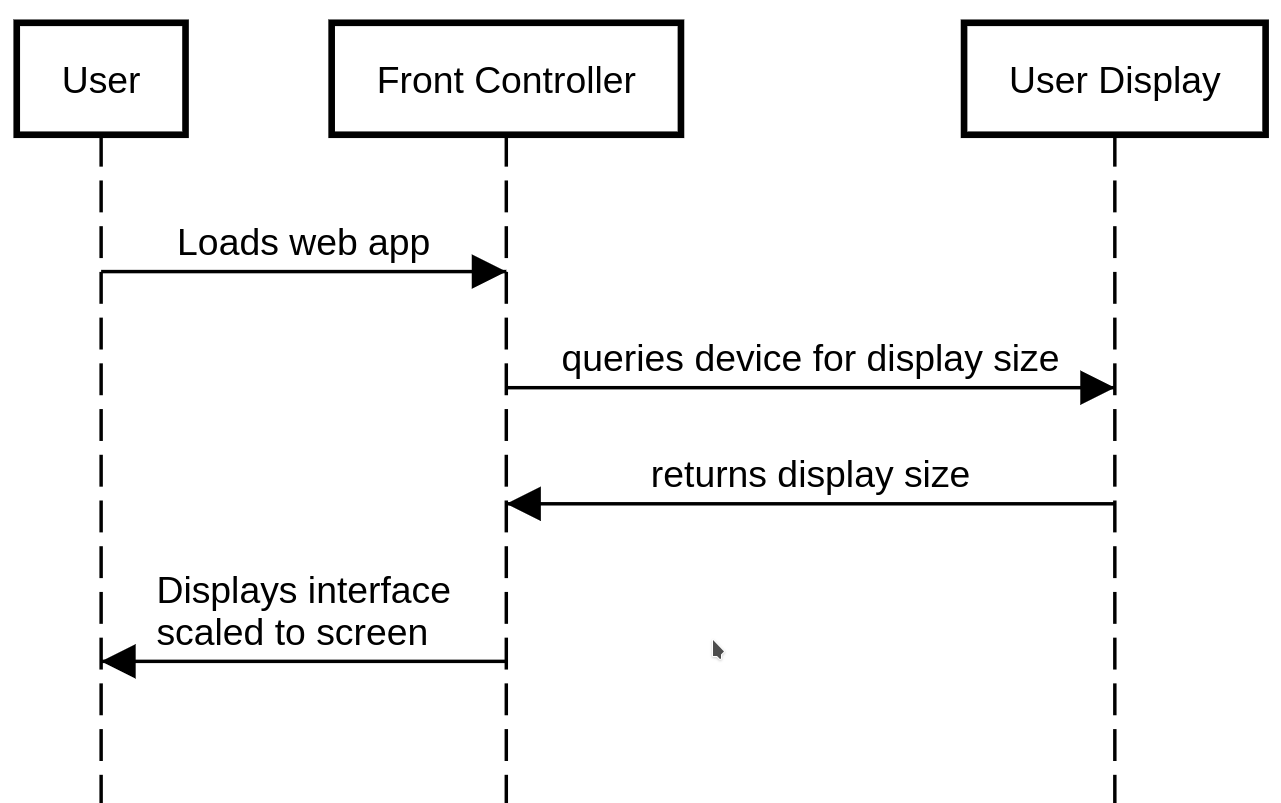
\includegraphics[scale=0.5]{img/responsive_web_page.png}\linebreak


\section{The Stories due Next Week}

Creating the web app to send and receive data into the server is the most
important part of the project. We have two groups, one working on frontend
(Aidan Grimshaw, Yufei Zeng, Ryan Sisco), and one on backend (Iliana Javier,
Brendan Byers). Communication is very important between the two teams, and
getting both parts to work together is the most important part.

The user stories that have the most priority, according to the customer, is “Add
a Post”, “Add a Comment”, and  “Like/Dislike”. These are needed in order to get
content onto the server, and get a starting point for the app. The rest of the
features should not be implemented until these 3 are completed. The frontend
team will develop the javascript and css according to our mockups. The backend
team will help handle importing the data and exporting the data. Error handling
will also be done according to the mockups.

The secondary tasks will be completed after the connection between the server
and user is more grounded and bug-free. Once that is true, development on the
tasks will begin. The backend team will handle receiving data from the user, and
the frontend team will develop the different pages needed for the tasks. Error
handling this data will not be as difficult, because there is no raw user input
to check. Security should be easiest on these as well, with little risk for a
dangerous bug here.

The estimated time till completion on the frontend is one week, on 3/1/18. This
should give lots of time to create a UI that looks very similar to the mockups.
The backend estimated time is 3/1/18 for proper communication between user and
server. Security will take longer, with no estimated time due to the long
process of investigated and auditing of our system. This means that the app will
have some functionality and be considered completed while security is still
being updated throughout the project. Getting our system working with data is
our top priority, and before all of these user stories can be done, this needs
to happen. This will be done with a simple webpage for testing with the
database. Security will have the task of checking user text and possible
attacks. This beginning code is the most vulnerable to malicious users, so it is
important that it works early on. After the communication is established, the
teams will be able to break off and continue development on their tasks. By
working this way, we believe that our project will work extremely well, and have
a complete backend and frontend that can be swapped if one or the other does not
work out, or if hosting becomes an issue.

\section{Meeting Report}

\subsection{Progress Made this Week}

This week we worked on gathering User Stories and planning their implementation.
We prioritized the 16 user stories into three categories: Due this week, due
next week, and reach goals. Each story was further partitioned into a list of
corresponding tasks to clarify how it will be implemented. To tackle
implementation we created Front End and Back End teams and divided the tasks
between them. We also divided the user story UML Sequence diagram creation
equally among the team members.

\subsection{Plans for Next Week}

Next week we will begin to code the highest priority stories, such as “Add a
Post”, “Add a Comment”, and “Like/Dislike”. We will be using the tools and
coding style we have documented in the past weeks to do so. Communication
between the Front and Back End teams will be emphasized to ensure all team
members are on the same page and code implementation can be as efficient as
possible.

\subsection{Team Member Contributions}

\begin{itemize}
  \item User Stories - Brendan Byers, Ryan Sisco, Iliana Javier Aiden Grimshaw
  \item Corresponding Tasks - Brendan Byers
  \item Stories Due Next Week - Ryan Sisco
  \item UML Sequence Diagrams - Ryan Sisco, Aiden Grimshaw, Yufei Zeng, Iliana Javier, Brendan Byers
  \item Meeting Report -  Iliana Javier
\end{itemize}

\end{document}
